\documentclass{bioinfo}
\copyrightyear{2014}
\pubyear{2014}

\usepackage{subfig}
\usepackage{listings}
\usepackage{ifthen}
\usepackage[english]{babel}
\usepackage[normalem]{ulem}
\usepackage{relsize}
\usepackage{rotate}
\usepackage{url}

\lstset{language=Java,
morendkeywords={String, Throwable}
captionpos=b,
basicstyle=\scriptsize\ttfamily,%\bfseries
stringstyle=\color{darkred}\scriptsize\ttfamily,
keywordstyle=\color{royalblue}\bfseries\ttfamily,
ndkeywordstyle=\color{forrestgreen},
numbers=left,
numberstyle=\scriptsize,
% backgroundcolor=\color{lightgray},
breaklines=true,
tabsize=2,
frame=single,
breakatwhitespace=true,
identifierstyle=\color{black},
% morecomment=[l][\color{forrestgreen}]{//},
% morecomment=[s][\color{lightblue}]{/**}{*/},
% morecomment=[s][\color{forrestgreen}]{/*}{*/},
commentstyle=\ttfamily\itshape\color{forrestgreen}
% framexleftmargin=5mm,
% rulesepcolor=\color{lightgray}
% frameround=ttff
}

% MACROS:

\newcommand{\TODO}[1]{\textcolor{red}{\textbf{#1}}}
\newcommand{\AbstractDESSolver}{\texttt{Abstract\-DES\-Solver}}
\newcommand{\OverdeterminationValidator}{\texttt{Overdetermination\-Validator}}
\newcommand{\SBMLinterpreter}{\texttt{SBML\-interpreter}}
\newcommand{\FirstOrderSolver}{\texttt{First\-Order\-Solver}}
\newcommand{\AbstractIntegrator}{\texttt{AbstractIntegrator}}
\newcommand{\MultiTable}{\texttt{Multi\-Table}}
\newcommand{\Block}{\texttt{Block}}
\newcommand{\jlibsedml}{\texttt{jlibsedml}}
\newcommand{\numero}{N\raisebox{.25em}{\relsize{-2}\underline{o}}}
\newcommand{\SBMLLaTeX}{{\sffamily\upshape\raisebox{-.35ex}{S\hspace{-.425ex}BML}\hspace{-0.5ex}2\LaTeX}}
%\begin{rotate}{-17.5}\raisebox{-.1ex}{2}\end{rotate}\hspace{1ex}\LaTeX}

\hyphenation{
  % TODO hypens for regular words
  im-ple-men-ta-tions
  gra-phi-cal
  bench-mark-ed
}

% some nice colors
\definecolor{royalblue}{cmyk}{.93, .79, 0, 0}
\definecolor{lightblue}{cmyk}{.10, .017, 0, 0}
\definecolor{forrestgreen}{cmyk}{.76, 0, .76, .45}
\definecolor{darkred}{rgb}{.7,0,0}
\definecolor{winered}{cmyk}{0,1,0.331,0.502}
\definecolor{lightgray}{gray}{0.97}

\graphicspath{{../../snapshot/}{../../../resources/org/sbml/squeezer/resources/img/}{img/}{img/SABIO-RK/}{img/icons/}}

\begin{document}
\firstpage{1}

\title[SBMLsqueezer~2]{SBMLsqueezer~2: a context-sensitive rate law generator for biochemical networks with access to SABIO-RK}
%versatile context-based generator of biochemical rate equations with access to SABIO-RK}
%for biochemical networks
\author[A.~Dr\"ager et~al.]{%
Andreas Dr\"ager\,$^{1,2,}$\footnote{to whom correspondence should be
addressed}\hspace{.3em},
Roland Keller\,$^{2}$,
Matthias Rall\,$^{2}$,
Johannes Eichner\,$^{2}$,
Bernhard \O. Palsson$^{1}$,
Andreas Zell\,$^{2}$}
\address{$^{1}$Systems Biology Research Group, University of California, San Diego, La Jolla, CA, United States
$^{2}$Center for Bioinformatics Tuebingen (ZBIT), University of Tuebingen, T\"ubingen, Germany}
\history{Received on XXXXX; revised on XXXXX; accepted on XXXXX}

\editor{Associate Editor: XXXXXXX}

\maketitle

\begin{abstract}
%\section{Motivation:}
\section{Summary:}
Modeling metabolic networks belongs to the most laborious and error-prone tasks in systems biology.
Size and complexity of published reconstructions are steadily increasing.
%The trend to move to personalized quantitative models requires the creation of patient-specific individual differential equation systems.
In order to simulate the dynamics of quantitative models, kinetic equations need to be derived for each reaction. Parameters and units also need to be specified.
%This work must be done for each individual reaction within the network.
The manual assignment of these equations is not practicable for large numbers of reactions.
Complex test-and-evaluation cycles require automated methods for rate law assignment.
%\section{Results:}
The program SBMLsqueezer~2 is a generator for kinetic equations, parameters, and units.
It distinguishes between multiple types of reactions and selects only suitable rate laws.
The user can influence all choices made by the program in order to assign the desired type of rate law to each reaction.
Experimentally derived rate laws can be obtained through a connection to the kinetics database SABIO-RK.
This platform-independent program can be used in a large variety of ways, enabling flexible solutions and use-case scenarios.
\section{Availability:}
Program, source code, and documentation can be obtained under the terms of the GPL version~3 from the website
\href{http://www.cogsys.cs.uni-tuebingen.de/software/SBMLsqueezer/}{http://www.cogsys.cs.uni-tuebingen.de/software/SBMLsqueezer/}.
\section{Contact:}
\href{mailto:sbmlsqueezer@googlegroups.com}{sbmlsqueezer@googlegroups.com}
%
%\section{Supplementary information:}
% TODO: Provide additional material
%Supplementary data is available at Bioinformatics online.
\end{abstract}

%\vspace{-.25cm}
\section{Introduction}

The reconstruction of genome-scale networks has been recognized as a highly laborious long-term effort, which requires several iterations of curation \citep{Thiele2010}.
However, for the creation of dynamic network simulations, the formulation of such a structural network is just the first step.
For each reaction within the network, a specific kinetic equation, a so-called rate law, needs to be derived.
These rate laws typically contain parameters, such as Michaelis constants, or even plain numbers, which are not always intended to be dimensionless quantities.
Reactive species in these models may cross compartments through transport reactions.
Hence, their reaction space may change and consequently their molarity with the volume differences of each compartment.
Ensuring unit consistency for the entire network requires careful consideration.
When a model is finally used as the basis for technical applications, inconsistent units could compromise 
therapeutic procedures or even endanger health and safety of patients.

Manually deriving both, kinetic equations and all units, brings several problems with it, because it
a) is highly error-prone, % opens the door for mistakes and errors
b) very time-consuming, and
c) cannot be applied in large-scale or automated approaches.
For these reasons, %it has been recognized that 
automatic procedures are required for the assembly of rate laws.
Programs, such as
COPASI \citep{Hoops2006}, 
CellDesigner \citep{Funahashi2007}, %\citep{Funahashi2003},
the MASS-Toolbox (\url{http://opencobra.github.io/MASS-Toolbox/}), and 
Cellerator \citep{Shapiro2002}, 
provide pre-defined lists of kinetic equations and also allow the user to modify these rate laws or to even create customized equations.
CellDesigner~4.3 %has only two pre-defined rate laws but 
provides a dialog that assists the user to obtain rate laws from the kinetics database SABIO-RK \citep{Wittig2012}.
The MASS-Toolbox focuses on the creation of elementary rate laws and automatically derives pseudo-elementary rate constants with their units.
Inference programs, such as Net\emph{Gene}rator \citep{Weber2013}, estimate a topology and generate specific rate laws  for gene-regulatory processes. 
Odefy \citep{Krumsiek2010} converts discrete Boolean networks into quantitative differential equation systems by applying Hill-type rate laws to each transition. % and creates parameters accordingly.
%COPASI version~4.12 gives the user the possibility to navigate through all reactions and to manually select an appropriate rate law to it from the list of currently 38 functions.
%Alternatively, the user can type a specific rate law or alter a given formula.
%CellDesigner version~4.3 provides two pre-defined rate laws, but also provides a text editor for customized formulas.
%CellDesigner has a dialog available that assists the user to obtain rate laws from the kinetics database SABIO-RK \citep{Wittig2012}.
%Cellerator \citep{Shapiro2002} facilitates equation generation by providing build-in functions for a set of rate laws, which the user can apply to reactions.

%SBMLsqueezer~2 has been implemented with the aim to simplify the difficult %and highly error-prone
%process of rate law assignment.
%The number of pre-defined rate laws is large and covers several aspects of research in systems biology.
In contrast, SBMLsqueezer~2 applies several criteria to automatically select appropriate equations for each reaction.
% of various types.
The user can influence these criteria %for this selection
and choose which rate law to apply.
The aims of this approach are
a) to ensure that only applicable rate laws can be selected and thus the consistency of the model, and
b) to reduce the required human interaction to a minimum.
SBMLsqueezer~2 is intended to be useful for modeling not only metabolic networks but also signal transduction processes and gene-regulatory mechanisms.


\vspace{-.1cm}
\section{Results}

Originally, SBMLsqueezer has been developed as a plug-in for CellDesigner \citep{Draeger2008}.
It was then extended to a %libSBML-based
stand-alone tool \citep{Draeger2010}.
SBMLsqueezer~2 can be used as
a) on-line program,
b) stand-alone tool via graphical user interface or command-line,
c) plug-in for CellDesigner,
d) Garuda gadget, and
e) through its API in complex workflows and algorithms.

The vast majority of biochemical reactions can be categorized into a limited number of classes.
SBMLsqueezer~2 takes several features of the reaction into account in order to discriminate these classes.
For each class it either determines all kinds of principally applicable rate laws, or the most suitable rate law.
The user can influence how rate laws are picked.
An equation preview assists the user to make this decision.
The program equips all newly generated parameters with units in order to ensure consistency.
It should be noted that for some levels and versions of SBML numbers cannot be associated with units and that some rate laws can under certain conditions not be evaluated to reaction extend per time units.

The dialog for access to SABIO-RK is similar to %the interface in CellDesigner and 
the on-line database service and %\citep{Funahashi2007}.
%This feature 
uses the annotation of the reaction and its components to identify the best match in SABIO-RK.
When successful, rate laws, parameters, units, and annotations will be transferred from SABIO-RK to the local model.
%
Rate law generation and extraction from SABIO-RK can be performed for individual reactions (fig.~\ref{fig:SBMLsqueezer}) or for the entire model in a single step.
%
Optionally, SBMLsqueezer~2 can remove unused variables and units from the model (cleaning) and update annotations where required.
The content of models can be summarized in a comprehensive human-readable PDF report.

\begin{figure}
\centering{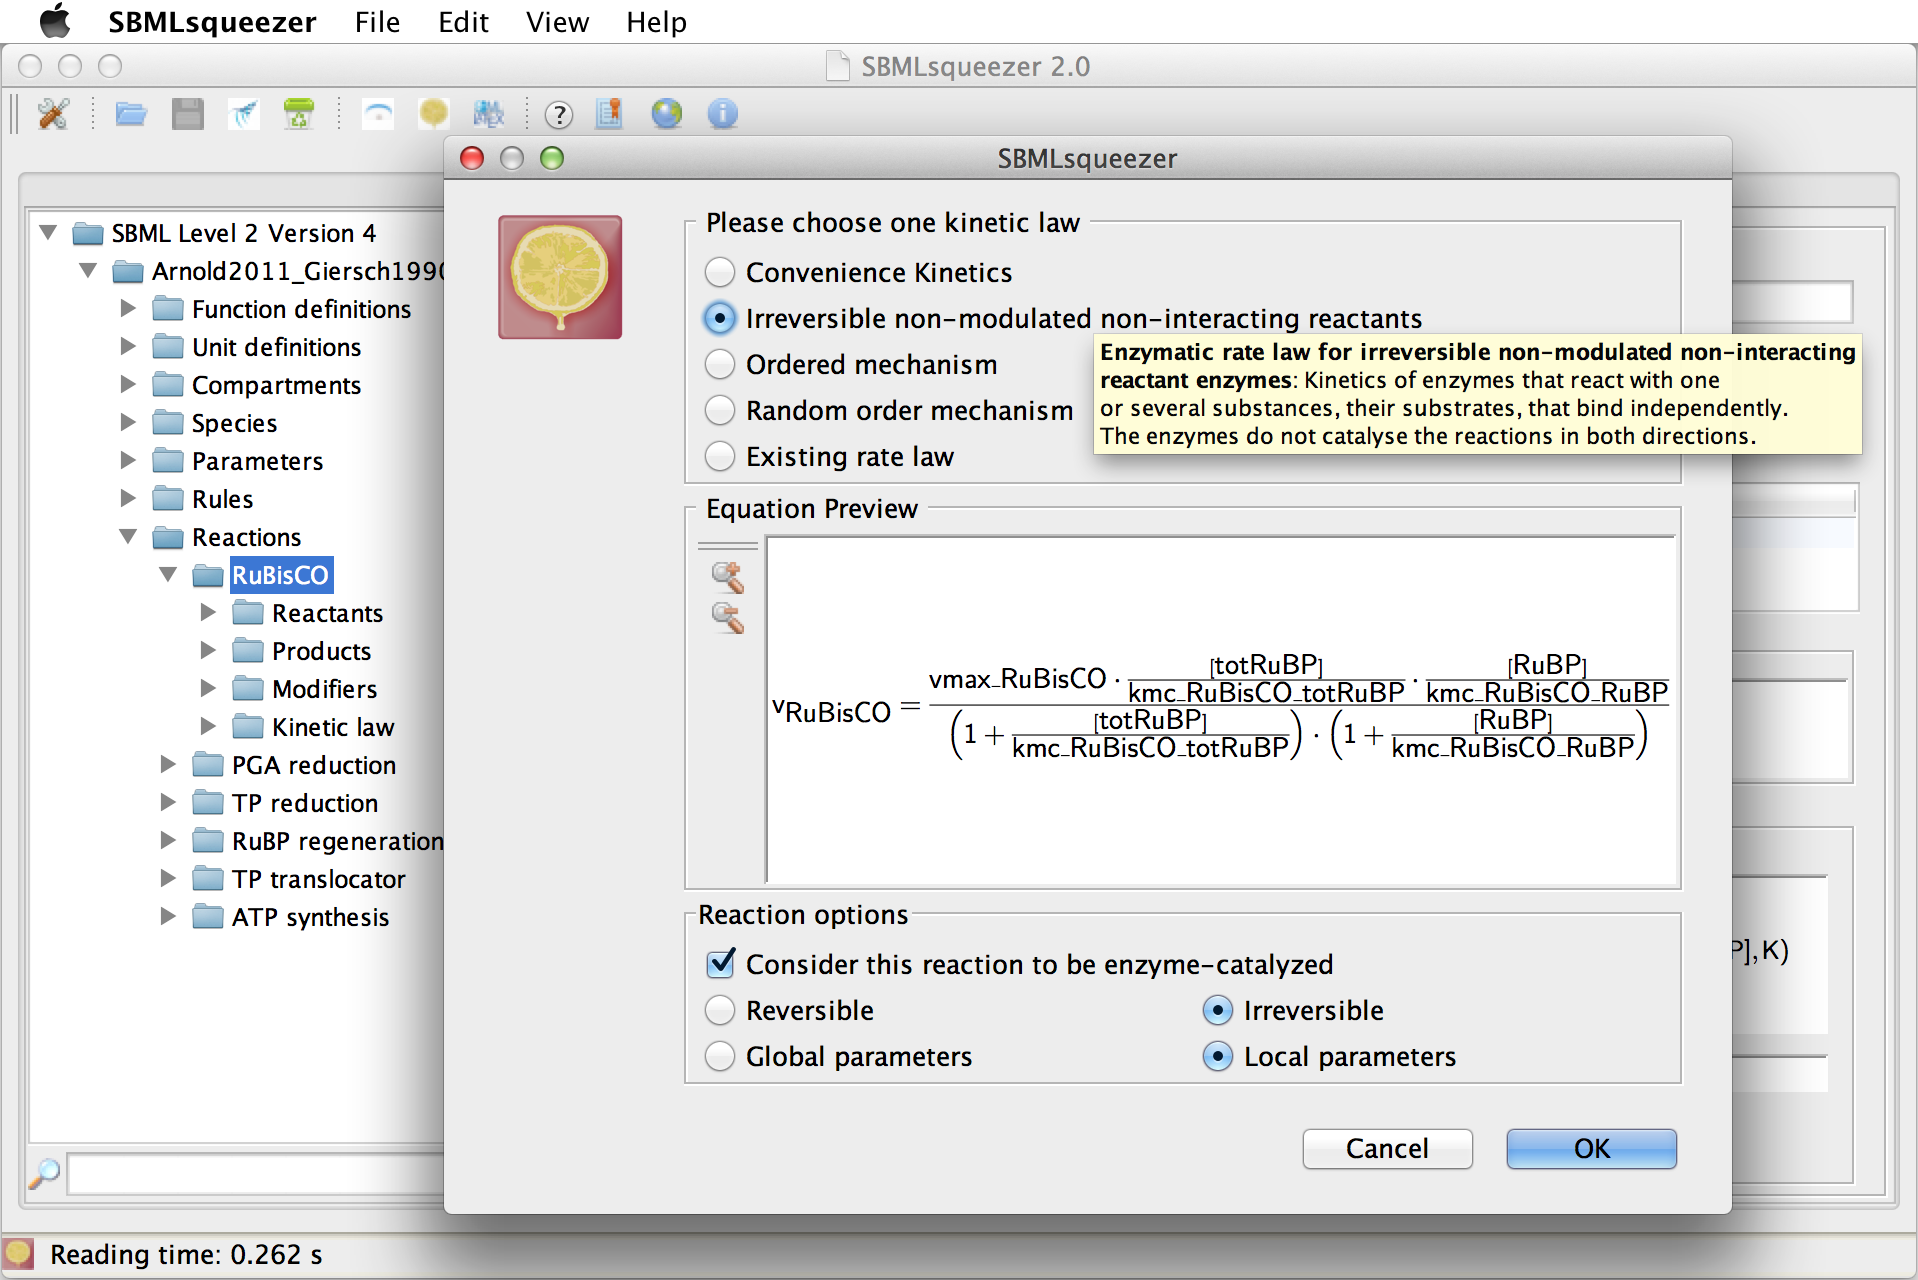
\includegraphics[width=.48\textwidth]{Screenshot_2.png}}
\caption[Reaction context dialog of SBMLsqueezer~2]{Reaction context dialog of SBMLsqueezer~2.}\label{fig:SBMLsqueezer}
\vspace{-.2cm}
\end{figure}

\vspace{-.45cm}
\begin{methods}
\section{Implementation}
SBMLsqueezer~2 is based on the data format SBML \citep{Hucka2004}.
It is entirely implemented in Java\texttrademark{} and runs on every platform, for which a JVM is available.
Reading and writing of SBML files is done with JSBML \citep{Draeger2011b}, which also acts as the internal data structure.
SBMLsqueezer~2 can also be launched using a libSBML \citep{Bornstein2008} back-end.
The on-line program version is based on the command-line interface of the stand-alone tool, which is wrapped in a Galaxy \citep{Goecks2010} framework.
For writing model reports, SBMLsqueezer~2 contains a development release of \SBMLLaTeX{} \citep{Draeger2009}.
The Garuda gadget \citep{Ghosh2011} is implemented based on the back-end API for Java\texttrademark.
The CellDesigner plug-in uses the communication interface between CellDesigner's plug-in API and JSBML.
Changes made by SBMLsqueezer~2 are synchronized with CellDesigner through a change listener interface.
SBMLsqueezer~2 determines the type of reaction by interpreting SBO and MIRIAM annotations \citep{Courtot2011} of all components as well as the number and kind of reaction participants.
Access to SABIO-RK \citep{Wittig2012} requires an active Internet connection and uses the RESTFUL API provided by SABIO-RK through a Java\texttrademark{} URL connection.
For detailed description of the algorithms, see the Users' Guide.
%SBMLsqueezer~2 has been internationalized and comes with language packs for German and English, and partially Chinese.
\end{methods}

%%%%%%%%%%%%%%%%%%%%%%%%%%%%%%%%%%%%%%%%%%%%%%%%%%%%%%%%%%%%%%%%%%%%%%%%%%%%%%%%%%%%%
%
%     please remove the " % " symbol from \centerline{\includegraphics{fig01.eps}}
%     as it may ignore the figures.
%
%%%%%%%%%%%%%%%%%%%%%%%%%%%%%%%%%%%%%%%%%%%%%%%%%%%%%%%%%%%%%%%%%%%%%%%%%%%%%%%%%%%%%%
%\vspace{-.01cm}
\section{Conclusion}

%SBMLsqueezer has been continuously developed since 2006.
With SBMLsqueezer~2 a mature and stable application has been released, which can be applied in diverse ways.
It can easily be integrated into versatile workflows and complex procedures.
The Users' Guide at the project web-site
% provides detailed information about 
explains in detail
how to exploit all program functions 
%SBMLsqueezer~2's API, all command-line options as well as 
and provides several sample use-cases.

%Efforts, such as the path2models project \citep{Buechel2013} were not possible without the availability of automated approaches for rate law assignment.
The path2models project \citep{Buechel2013} has demonstrated the usefulness of automated rate law assignment.
%Complex try-and-evaluate cycles, in which the most suitable rate law for a certain reaction needs to be identified in repeated simulation runs, also require such a method \citep{Draeger2011}.
Based on SBMLsqueezer~2
%this program, 
complex try-and-evaluate cycles, in which the most suitable rate law for a certain reaction needs to be identified in repeated simulation runs \citep{Draeger2011} now become possible.

\vspace{-.2cm}
\section*{Acknowledgments}

The authors are grateful to Meike Aichele, Hannes Borch, Alexander D\"orr, Martin Golebiewski, Nadine Hassis, Marcel Kronfeld, Oliver Kohlbacher, Wolfgang M\"uller, Sarah R.~M\"uller vom Hagen, Sebastian Nagel, Leif J.~Pallesen, Alexander Peltzer, Julianus Pfeuffer, Sandra Saliger, Simon Sch\"afer, Adrian Schr\"oder, Jochen Supper, Dieudonn\'e M.~Wouamba, Shaowu Yang, Michael J.~Ziller.
%The authors are grateful to M.~Aichele, H.~Borch, A.~D\"orr, M. Golebiewski, N.~Hassis, M.~Kronfeld, O.~Kohlbacher, W.~M\"uller, S. R. M\"uller vom Hagen, S.~Nagel, L.~J.~Pallesen, A.~Peltzer, J. Pfeuffer, S.~Saliger, S.~Sch\"afer, A.~Schr\"oder, J.~Supper, D. M. Wouamba, S. Yang, and M.~J.~Ziller.

%\vspace{-.05cm}
\paragraph{Funding\textcolon}
Thanks to the Federal Ministry of Education and Research (BMBF, Germany) for funding the
Virtual Liver Network (grant number 0315756) and to %the European Commission for granting 
the 7\textsuperscript{th} EU Framework Program for Research and Technological Development
for AD's Marie Curie International Outgoing Fellowship
(project AMBiCon, 332020).

%\vspace{-.05cm}
\paragraph{Conflict of Interest\textcolon} none declared.

\vspace{-.2cm}
%\bibliographystyle{natbib}
%\bibliography{document}

\begin{thebibliography}{}
\newcommand{\Bioinformatics}{Bioinformatics}
\bibitem[Bornstein {\em et~al.}(2008)Bornstein {\em et~al.}]{Bornstein2008}
Bornstein {\em et~al.} (2008).
\newblock {LibSBML: an API library for SBML}.
\newblock {\em \Bioinformatics\/}, {\bf 24}(6), 880--881.

\bibitem[B{\"u}chel {\em et~al.}(2013)B{\"u}chel {\em et~al.}]{Buechel2013}
B{\"u}chel {\em et~al.} (2013).
\newblock Large-scale generation of computational models from biochemical
  pathway maps.
\newblock {\em BMC Syst Biol\/}, {\bf 7}(1), 116.

\bibitem[Courtot {\em et~al.}(2011)Courtot {\em et~al.}]{Courtot2011}
Courtot {\em et~al.} (2011).
\newblock Controlled vocabularies and semantics in systems biology.
\newblock {\em Mol Syst Biol\/}, {\bf 7}, 543.

\bibitem[Dr{\"a}ger(2011)Dr{\"a}ger]{Draeger2011}
Dr{\"a}ger, A. (2011).
\newblock {\em {Computational Modeling of Biochemical Networks}\/}.
\newblock Ph.D. thesis, University of Tuebingen.

\bibitem[Dr{\"a}ger {\em et~al.}(2008)Dr{\"a}ger {\em et~al.}]{Draeger2008}
Dr{\"a}ger, {\em et~al.} (2008).
\newblock {SBMLsqueezer: a CellDesigner plug-in to generate kinetic rate
  equations for biochemical networks}.
\newblock {\em BMC Syst Biol\/}, {\bf 2}(1), 39.

%\bibitem[Dr{\"a}ger {\em et~al.}(2009a)Dr{\"a}ger {\em et~al.}]{Draeger2009a}
%Dr{\"a}ger {\em et~al.} (2009a).
%\newblock {Modeling metabolic networks in \emph{C.~glutamicum}: a comparison of
%  rate laws in combination with various parameter optimization strategies}.
%\newblock {\em BMC Syst Biol\/}, {\bf 3}, 5.

\bibitem[Dr{\"a}ger {\em et~al.}(2009)Dr{\"a}ger {\em et~al.}]{Draeger2009}
Dr{\"a}ger {\em et~al.} (2009).
\newblock {SBML2\LaTeX: Conversion of SBML files into human-readable reports}.
\newblock {\em \Bioinformatics\/}, {\bf 25}(11), 1455--1456.

\bibitem[Dr{\"a}ger {\em et~al.}(2010)Dr{\"a}ger {\em et~al.}]{Draeger2010}
Dr{\"a}ger {\em et~al.} (2010).
\newblock {\em Systems Biology for Signaling Networks\/}, volume~2, chap.
  Automating mathematical modeling of biochemical reaction networks.
\newblock Springer.

\bibitem[Dr{\"a}ger {\em et~al.}(2011)Dr{\"a}ger {\em et~al.}]{Draeger2011b}
Dr{\"a}ger {\em et~al.} (2011).
\newblock {JSBML: a flexible Java library for working with SBML}.
\newblock {\em \Bioinformatics\/}, {\bf 27}(15), 2167--2168.

%\bibitem[Funahashi {\em et~al.}(2003)Funahashi {\em et~al.}]{Funahashi2003}
%Funahashi {\em et~al.} (2003).
%\newblock {CellDesigner: a process diagram editor for gene-regulatory and
%  biochemical networks}.
%\newblock {\em BioSilico\/}, {\bf 1}(5), 159--162.

\bibitem[Funahashi {\em et~al.}(2007)Funahashi {\em et~al.}]{Funahashi2007}
Funahashi {\em et~al.} (2007).
\newblock {Integration of CellDesigner and SABIO-RK}.
\newblock {\em In Silico Biology\/}, {\bf 7}(2 Suppl), S81--S90.

\bibitem[Ghosh {\em et~al.}(2011)Ghosh {\em et~al.}]{Ghosh2011}
Ghosh {\em et~al.} (2011).
\newblock Software for systems biology: from tools to integrated platforms.
\newblock {\em Nat Rev Genet\/}, {\bf 12}(12), 821--832.

\bibitem[Goecks {\em et~al.}(2010)Goecks {\em et~al.}]{Goecks2010}
Goecks {\em et~al.} (2010).
\newblock Galaxy: a comprehensive approach for supporting accessible,
  reproducible, and transparent computational research in the life sciences.
\newblock {\em Genome Biol\/}, {\bf 11}(8), R86.

\bibitem[Hoops {\em et~al.}(2006)Hoops {\em et~al.}]{Hoops2006}
Hoops {\em et~al.} (2006).
\newblock {COPASI--a COmplex PAthway SImulator}.
\newblock {\em \Bioinformatics\/}, {\bf 22}(24), 3067--3074.

\bibitem[Hucka {\em et~al.}(2004)Hucka {\em et~al.}]{Hucka2004}
Hucka {\em et~al.} (2004).
\newblock {Evolving a \emph{lingua franca} and associated software
  infrastructure for computational systems biology: the Systems Biology Markup
  Language (SBML) project}.
\newblock {\em Systems Biology, IEE\/}, {\bf 1}(1), 41--53.

\bibitem[Krumsiek {\em et~al.}(2010)Krumsiek {\em et~al.}]{Krumsiek2010}
Krumsiek {\em et~al.} (2010).
\newblock Odefy--from discrete to continuous models.
\newblock {\em BMC \Bioinformatics\/}, {\bf 11}, 233.

\bibitem[Shapiro {\em et~al.}(2002)Shapiro {\em et~al.}]{Shapiro2002}
Shapiro {\em et~al.} (2002).
\newblock Cellerator: extending a computer algebra system to include
  biochemical arrows for signal transduction simulations.
\newblock {\em \Bioinformatics\/}, {\bf 19}(5), 677--678.

\bibitem[Thiele and Palsson(2010)Thiele and Palsson]{Thiele2010}
Thiele, I. and Palsson, B.~{\O}. (2010).
\newblock A protocol for generating a high-quality genome-scale metabolic
  reconstruction.
\newblock {\em Nat Protoc\/}, {\bf 5}(1), 93--121.

\bibitem[Weber {\em et~al.}(2013)Weber {\em et~al.}]{Weber2013}
Weber {\em et~al.} (2013).
\newblock Inference of dynamical gene-regulatory networks based on
  time-resolved multi-stimuli multi-experiment data applying Net\emph{Gene}rator v2.0.
\newblock {\em BMC Syst Biol\/}, {\bf 7}(1), 1.

\bibitem[Wittig {\em et~al.}(2012)Wittig {\em et~al.}]{Wittig2012}
Wittig {\em et~al.} (2012).
\newblock {SABIO-RK--database for biochemical reaction kinetics}.
\newblock {\em Nucleic Acids Res\/}, {\bf 40}(Database issue), D790--D796.

\end{thebibliography}


\end{document}
